\begin{flushleft}
	\section{\textcolor{cyan}{Les technologies utilisés dans le projet}}
	\subsection{\textcolor{green}{Arduino Nano :}}
	\begin{figure}[h]
		\begin{minipage}{0.6\textwidth}
		L'Arduino Nano est un microcontrôleur programmable qui utilise une puce ATMega328P. Il dispose d'une horloge à quartz, de 14 broches d'entrée/sortie numériques, de 6 broches d'entrée analogiques, d'un régulateur de tension et d'une interface USB pour la programmation et la communication.
		
		Le microcontrôleur utilise également diverses technologies pour permettre la communication et le contrôle des composants connectés à ses broches, telles que:
		
		I2C (Inter-Integrated Circuit) pour la communication avec les capteurs et les autres dispositifs.
		SPI (Serial Peripheral Interface) pour la communication avec les écrans LCD, les cartes SD et autres périphériques.
		PWM (Pulse Width Modulation) pour générer des signaux analogiques à partir des broches numériques.
		UART (Universal Asynchronous Receiver/Transmitter) pour la communication série avec d'autres dispositifs.
		
		\end{minipage}
		\begin{minipage}{0.4\textwidth}
			\centering
			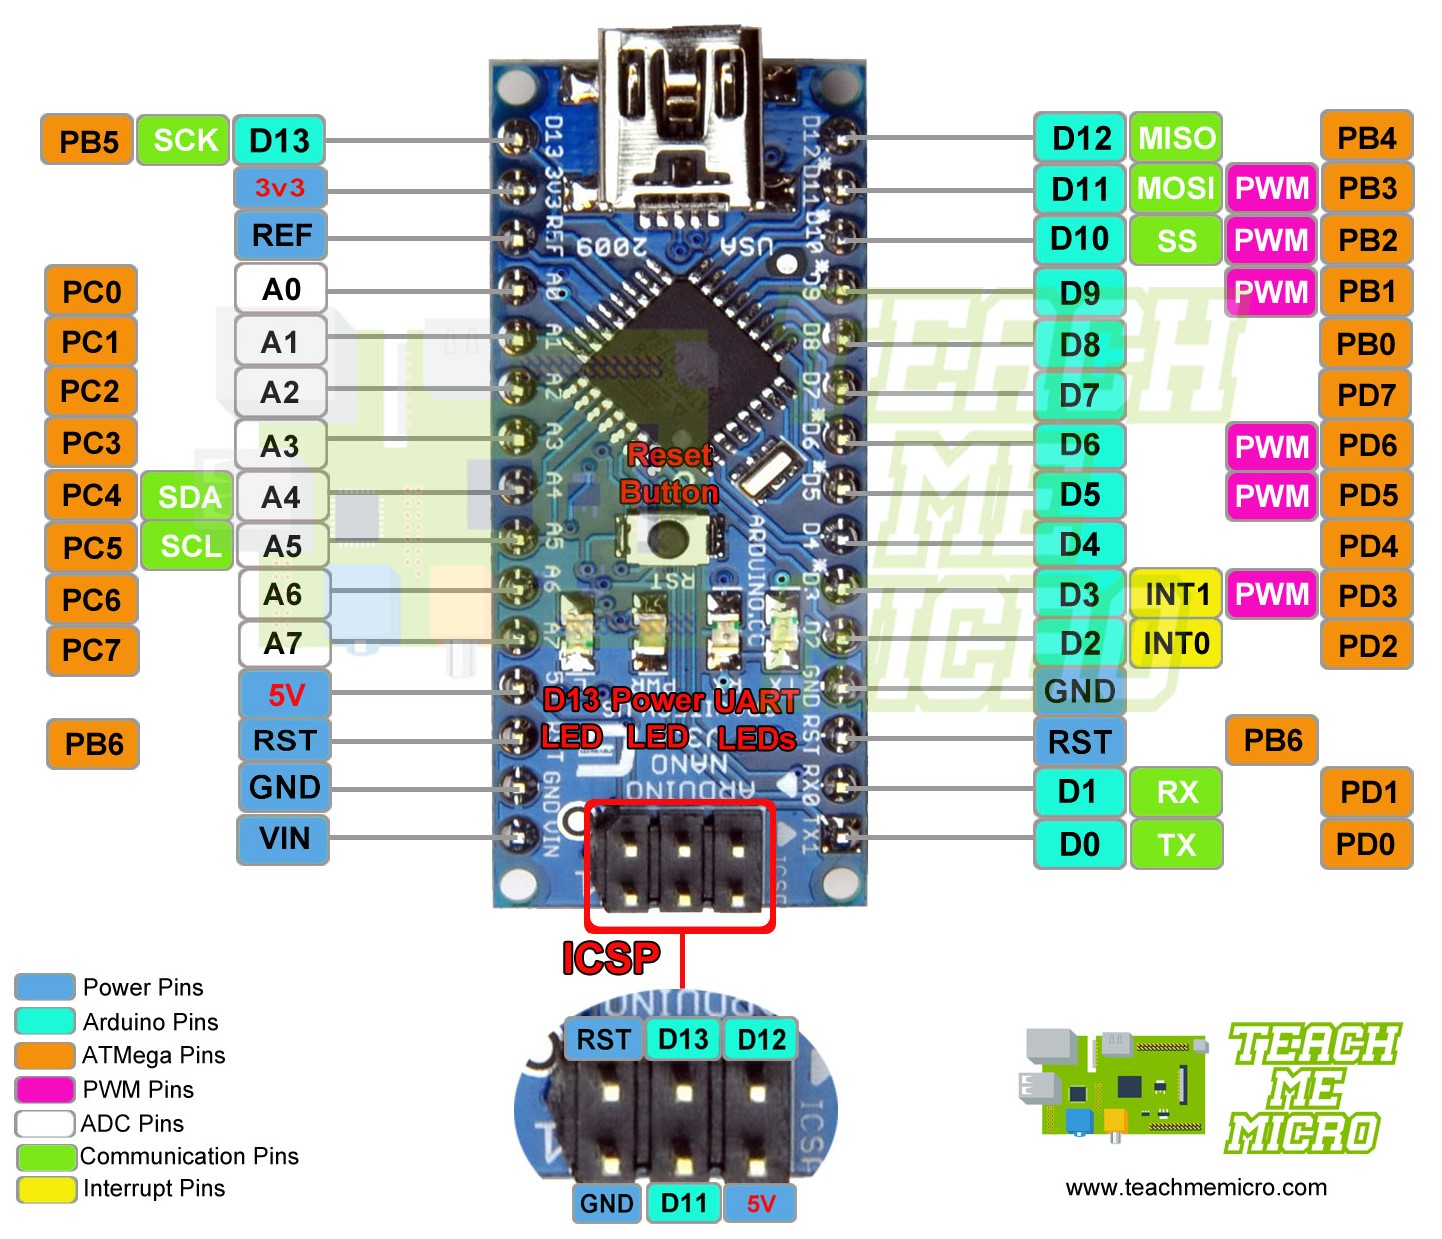
\includegraphics[width=\textwidth]{chapitres/images/Arduino-Nano-pinout.jpg}
			\caption{Arduino Nano}
			\label{fig:votre_image}
		\end{minipage}
	\end{figure}
	\subsection{\textcolor{green}{La carte NodeMCU :}}
		\begin{figure}[h]
			\begin{minipage}{0.6\textwidth}
				L'ESP8266 est un microcontrôleur Wi-Fi très populaire, souvent utilisé pour les projets d'IoT et les objets connectés. Il intègre un processeur Tensilica Xtensa LX106, une mémoire flash et une connectivité Wi-Fi.
				
				Les principales technologies utilisées dans l'ESP8266 sont:
				
				Wi-Fi : L'ESP8266 est équipé d'un module Wi-Fi intégré qui prend en charge les normes IEEE 802.11 b/g/n, offrant ainsi une connectivité sans fil pour les projets d'IoT.
				GPIO (General Purpose Input/Output) : L'ESP8266 dispose de plusieurs broches GPIO qui peuvent être utilisées pour contrôler des périphériques externes ou recevoir des signaux d'entrée.
				ADC (Analog-to-Digital Converter) : L'ESP8266 dispose d'un convertisseur analogique-numérique intégré pour mesurer des signaux analogiques.
				PWM (Pulse Width Modulation) : L'ESP8266 prend en charge la génération de signaux PWM sur certaines de ses broches pour contrôler des composants tels que des LED ou des moteurs.
				I2C (Inter-Integrated Circuit) : L'ESP8266 prend en charge la communication via le protocole I2C pour se connecter à des capteurs, des afficheurs et d'autres périphériques.
				SPI (Serial Peripheral Interface) : L'ESP8266 prend également en charge le protocole SPI pour communiquer avec des périphériques tels que des écrans LCD, des cartes SD et d'autres modules.
			\end{minipage}
			\begin{minipage}{0.4\textwidth}
				\centering
				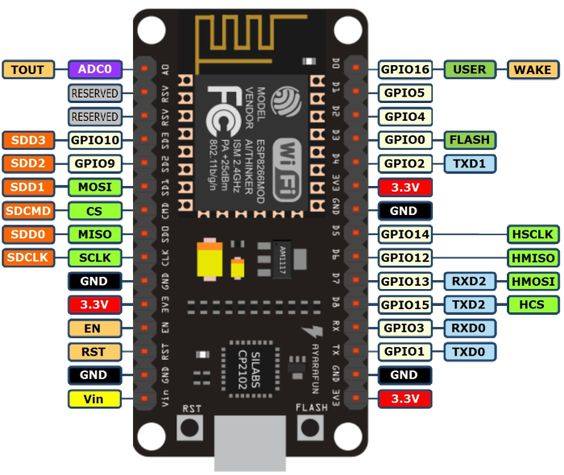
\includegraphics[width=\textwidth]{chapitres/images/esp8266.jpg}
				\caption{La carte NodeMCU}
				\label{fig:votre_image}
			\end{minipage}
		\end{figure}
	\newpage
	\subsection{\textcolor{green}{Le capteur DHT11 :}}
		\begin{figure}[h]
			\begin{minipage}{0.6\textwidth}
				Le capteur DHT11 est un capteur d'humidité et de température numérique très couramment utilisé dans les projets électroniques et les systèmes d'automatisation. Il utilise un élément de mesure d'humidité capacitif et un thermistor pour mesurer l'humidité relative et la température ambiante.
				
				Le DHT11 est capable de mesurer l'humidité relative dans une plage de 20\% à 90\% avec une précision de ± 5\%, et la température dans une plage de 0 à 50 degrés Celsius avec une précision de ± 2 degrés Celsius. Il est facile à utiliser car il ne nécessite que trois broches pour l'interfaçage avec un microcontrôleur ou une carte de développement.
				
				Cependant, il est important de noter que le DHT11 peut être affecté par l'interférence électromagnétique et peut avoir des mesures inexactes lorsqu'il est utilisé dans des environnements très humides ou très secs. De plus, il a une faible fréquence d'échantillonnage et peut prendre jusqu'à 2 secondes pour fournir des lectures précises, ce qui peut être un inconvénient dans certaines applications en temps réel
			\end{minipage}
			\begin{minipage}{0.4\textwidth}
				\centering
				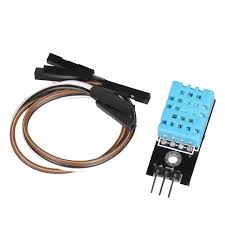
\includegraphics[width=\textwidth]{chapitres/images/dht11.jpg}
				\caption{Le capteur DHT11}
				\label{fig:votre_image}
			\end{minipage}
		\end{figure}
	\subsection{\textcolor{green}{Le capteur d’humidité de sol YL-69 :}}
		\begin{figure}[h]
			\begin{minipage}{0.6\textwidth}
				Le capteur d'humidité de sol YL-69 est un capteur simple et économique qui permet de mesurer l'humidité du sol. Il est souvent utilisé dans des projets d'irrigation automatique, de jardinage et de surveillance de la croissance des plantes.
				
				Le capteur YL-69 fonctionne en mesurant la résistance électrique du sol, qui varie en fonction de son humidité. Il est équipé de deux broches qui doivent être insérées dans le sol. Lorsque le sol est sec, la résistance est élevée et lorsque le sol est humide, la résistance est faible.
				
				Le capteur YL-69 est compatible avec une large gamme de microcontrôleurs tels que Arduino, Raspberry Pi, etc. Il est facile à utiliser car il ne nécessite que deux broches pour l'interfaçage avec le microcontrôleur.
			\end{minipage}
			\begin{minipage}{0.4\textwidth}
				\centering
				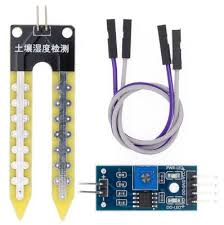
\includegraphics[width=\textwidth]{chapitres/images/siol-sensor.jpg}
				\caption{Le capteur d’humidité de sol YL-69}
				\label{fig:votre_image}
			\end{minipage}
		\end{figure}
	\newpage
	\subsection{\textcolor{green}{La photorésistance (LDR) :}}
		\begin{figure}[h]
			\begin{minipage}{0.6\textwidth}
				La photorésistance (LDR), également connue sous le nom de résistance sensible à la lumière, est un capteur de lumière passif qui varie sa résistance électrique en fonction de l'intensité lumineuse. Elle est souvent utilisée dans les systèmes d'automatisation, les projets électroniques et les dispositifs d'éclairage.
				
				La LDR est un composant électronique passif, ce qui signifie qu'elle ne nécessite pas d'alimentation électrique pour fonctionner. Elle est composée d'un matériau semi-conducteur qui varie sa résistance électrique en fonction de la quantité de lumière incidente. Lorsque la LDR est exposée à une forte intensité lumineuse, sa résistance diminue et lorsque la lumière est faible, sa résistance augmente.
				
				La LDR peut être utilisée pour détecter la présence ou l'absence de lumière, ou pour mesurer l'intensité de la lumière ambiante. Elle est souvent utilisée dans des applications telles que les circuits de commande de lumière automatiques, les capteurs de mouvement, les alarmes de sécurité et les systèmes de contrôle de l'exposition dans la photographie.
			\end{minipage}
			\begin{minipage}{0.4\textwidth}
				\centering
				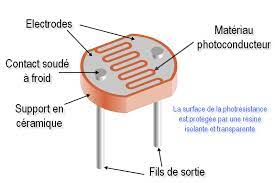
\includegraphics[width=\textwidth]{chapitres/images/ldr.jpg}
				\caption{La photorésistance (LDR)}
				\label{fig:votre_image}
			\end{minipage}
		\end{figure}
	\subsection{\textcolor{green}{Le capteur de niveau d’eau ST045 :}}
		\begin{figure}[h]
			\begin{minipage}{0.6\textwidth}
				Le capteur de niveau d'eau ST045 est un capteur de pression fabriqué par Shinesky Electronics Co., Ltd. Il est utilisé pour mesurer le niveau d'eau dans les réservoirs, les puits, les rivières, les lacs et autres conteneurs d'eau. Le capteur utilise la technologie de mesure de pression pour mesurer la hauteur de l'eau et convertir cette mesure en une sortie de signal électrique standard.
				
				Les caractéristiques du capteur ST045 incluent un corps en acier inoxydable, une plage de mesure de 0-5m à 0-200m, une précision de ±0,5\% FS, une température de fonctionnement de -10°C à 70°C, une tension d'alimentation de 9-36VDC et une sortie de signal de 4-20mA ou 0-5VDC.
			\end{minipage}
			\begin{minipage}{0.4\textwidth}
				\centering
				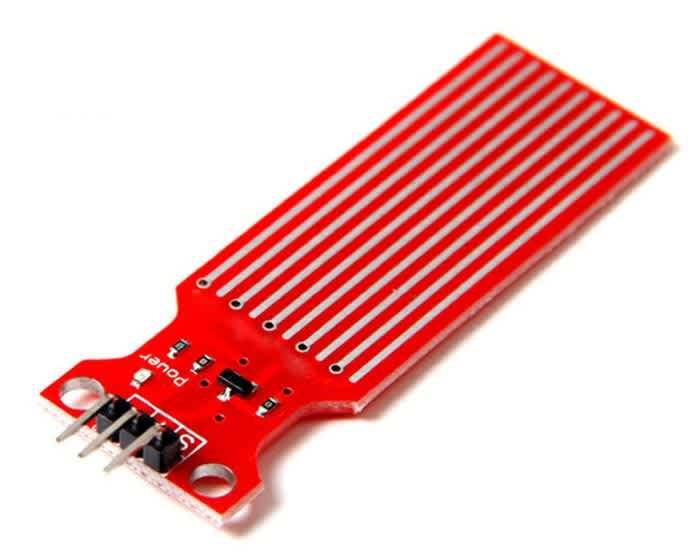
\includegraphics[width=\textwidth]{chapitres/images/waterlevelsensor.jpg}
				\caption{Le capteur de niveau d’eau ST045}
				\label{fig:votre_image}
			\end{minipage}
		\end{figure}
	\newpage
	\subsection{\textcolor{green}{Relais électrique SRD-05VDC-SL-C :}}
		\begin{figure}[h]
			\begin{minipage}{0.6\textwidth}
				Le relais électrique SRD-05VDC-SL-C est un relais de puissance de la série SRD fabriqué par Songle Relay. Il est utilisé pour contrôler les circuits électriques à partir d'un signal de commande électrique. Le relais est constitué d'une bobine de commande, de contacts électriques et d'un boîtier en plastique.
				
				La bobine de commande du relais est alimentée par une tension continue de 5VDC et lorsqu'elle est activée, elle attire un contacteur qui permet de fermer ou d'ouvrir un circuit électrique. Le relais est équipé de contacts à commutation inverse qui permettent de commuter des charges à la fois en courant alternatif (AC) et en courant continu (DC).
				
				Le relais SRD-05VDC-SL-C est largement utilisé dans diverses applications industrielles et domestiques, telles que le contrôle de l'éclairage, le contrôle des ventilateurs, le contrôle des moteurs, le contrôle des systèmes de climatisation, le contrôle des portes automatiques et bien d'autres encore.
				
			\end{minipage}
			\begin{minipage}{0.4\textwidth}
				\centering
				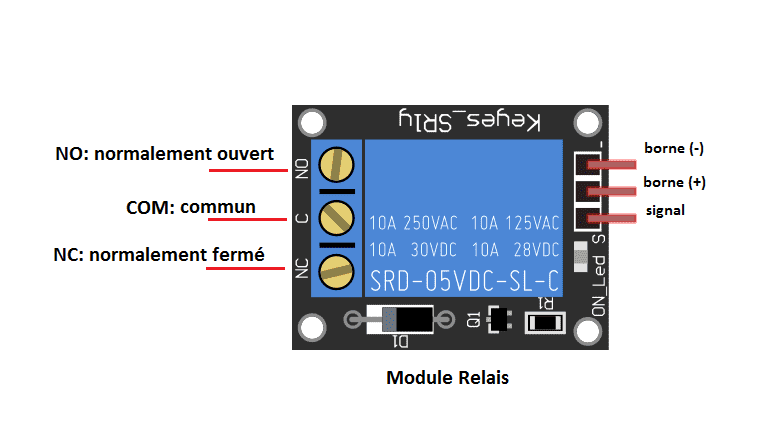
\includegraphics[width=\textwidth]{chapitres/images/relai-2-1.png}
				\caption{Relais électrique SRD-05VDC-SL-C}
				\label{fig:votre_image}
			\end{minipage}
		\end{figure}
	\subsection{\textcolor{green}{Mini Pompe DC 3-5V 70-120L/H :}}
		\begin{figure}[h]
			\begin{minipage}{0.6\textwidth}
				Cette pompe submersible va permettre de pomper de l’eau avec un débit de 70 à 120 l/h en fonction de l’alimentation de 3 à 5V.
				Caractéristiques
				
				\begin{itemize}
					\item Alimentation : 3 à 5V	
					\item 				Consommation : 100 à 200 mA	
					\item 				Débit : 10 à 120 l/h
				\end{itemize}
			\end{minipage}
			\begin{minipage}{0.4\textwidth}
				\centering
				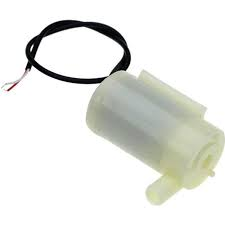
\includegraphics[width=\textwidth]{chapitres/images/pompe.jpg}
				\caption{Mini Pompe DC 3-5V 70-120L/H}
				\label{fig:votre_image}
			\end{minipage}
		\end{figure}
	
	
	\newpage
\end{flushleft}